% !TEX program=lualatex
\documentclass[12pt,letterpaper]{article}

\usepackage[letterpaper,margin=1in]{geometry}

\usepackage{amsmath}
\usepackage{amssymb}
\usepackage{mathtools}
\usepackage[warnings-off={mathtools-colon,mathtools-overbracket}]{unicode-math}
\usepackage{fontspec}
\usepackage{microtype}

\setmainfont{TeX Gyre Pagella}
\setmathfont{Latin Modern Math}

\usepackage{url}
\usepackage{graphicx}

\usepackage[compact,tiny]{titlesec}

\usepackage[authoryear,round]{natbib}

\usepackage{tikz}
\usetikzlibrary{arrows,automata,positioning,shapes,decorations.text,backgrounds,matrix}
\usepackage{wrapfig, framed}
\usepackage[font=small,labelfont=bf]{caption}
\usepackage[hidelinks]{hyperref}
\usepackage{listings}
\usepackage{relsize}
\usepackage[left]{lineno}
\usepackage{colortbl}
\usepackage{multicol}

\pagenumbering{arabic}
\newcommand*\pct{\scalebox{.9}{\%}}
\newcommand{\red}[1]{\textcolor{red}{#1}}
\newcommand{\green}[1]{\textcolor{green}{#1}}
\newcommand{\cyan}[1]{\textcolor{cyan}{#1}}
\newcommand{\grande}[1]{\mathlarger{\mathlarger{#1}}}

\hypersetup{
    colorlinks=true,
    linkcolor=black,
    urlcolor=blue,
    citecolor=black
}

\newcommand{\TODO}[1]{\begingroup\bfseries\color{red}TODO:~#1\endgroup}

% document begins here
\begin{document}
% title goes here:
\begin{flushleft}
{\Large\textbf{COATi: statistical pairwise alignment of protein-coding sequences}}
\newline
% authors go here:
\\
Juan J. García Mesa\textsuperscript{1,2},
Ziqi Zhu\textsuperscript{1,3},
Reed A. Cartwright\textsuperscript{1,3,*}\\
\bigskip
1 The Biodesign Institute, Arizona State University, Tempe, Arizona, USA\\
2 Ira A.\ Fulton Schools of Engineering, Arizona State University, Tempe, Arizona, USA\\
3 School of Life Sciences, Arizona State University, Tempe, Arizona, USA\\
\bigskip
* cartwright@asu.edu

\end{flushleft}

\begin{abstract}
\noindent
Sequence alignment is an essential method in bioinformatics and the basis of many analyses, including phylogenetic inference, ancestral sequence reconstruction, and gene annotation. Sequence artifacts and errors made in alignment reconstruction can impact downstream analyses leading to erroneous conclusions in comparative and functional genomic studies. For example, abiological frameshifts and early stop codons are common artifacts found in protein coding sequences that have been annotated in reference genomes. While such errors are eventually fixed in the reference genomes of model organisms, many genomes used by researchers contain these artifacts, and researchers often discard large amounts of data in comparative genomic studies to prevent artifacts from impacting results. To address this need, we present COATi, a statistical, codon-aware pairwise aligner that supports complex insertion-deletion models and can handle artifacts present in genomic data. COATi allows users to reduce the amount of discarded data while generating more accurate sequence alignments.
\end{abstract}

% now start line numbers
\linenumbers

\section*{Introduction}

Sequence alignment is a fundamental task in bioinformatics and a cornerstone step in comparative and functional genomic analysis \citep{sequence_alignment_rosenberg_2009}. While sophisticated advancements have been made, the challenge of alignment inference has not been fully solved \citep{art_morrison_2015}.
%Modern sequence analysis began with the heuristic homology algorithms of \textcite{Needleman1970} and \textcite{identification_smith_1981} and, while the methods developed since then have improved, alignment inference is not a solved problem \citep{art_morrison_2015}. 
%
The alignment of protein-coding DNA sequences is one such challenge, and a common approach to this problem is to perform alignment inference in amino-acid space \citep[e.g.][]{bininda2005transalign,abascal2010translatorx}. While this approach is an improvement over DNA models, it discards information, underperforms compared to alignment at the codon level, and fails in the presence of artifacts, such as frameshifts and early stop codons. While some aligners can utilize codon substitution models, they are often not robust against coding-sequence artifacts.

Within protein-coding sequences, indels may occur in between any pair of adjacent nucleotides, and therefore, gaps in alignments of natural sequences may occur both between and within codons (Fig.\ \ref{fig:aln}). Gaps that occur after the first position or second position of a codon are known as phase-1 and phase-2 gaps, respectively. Gaps that occur between codons are known as either phase-3 gaps (this study) or phase-0 gaps \citep[e.g.][]{taylor2004occurrence}. While all three phases of gaps occur in natural sequences, alignments performed in amino-acid or codon space force all gaps to be phase-3 gaps. Because only about 42\% of indels are phase-3 \citep{taylor2004occurrence, zhu2022profiling}, this mismatch between aligner assumptions and biology can produce sub-optimal alignments and inflated estimates of sequence divergence (Fig.\ \ref{fig:aln}).

% Figures are 86 mm or 178 mm wide
\begin{figure}[h!]
    \centering%
    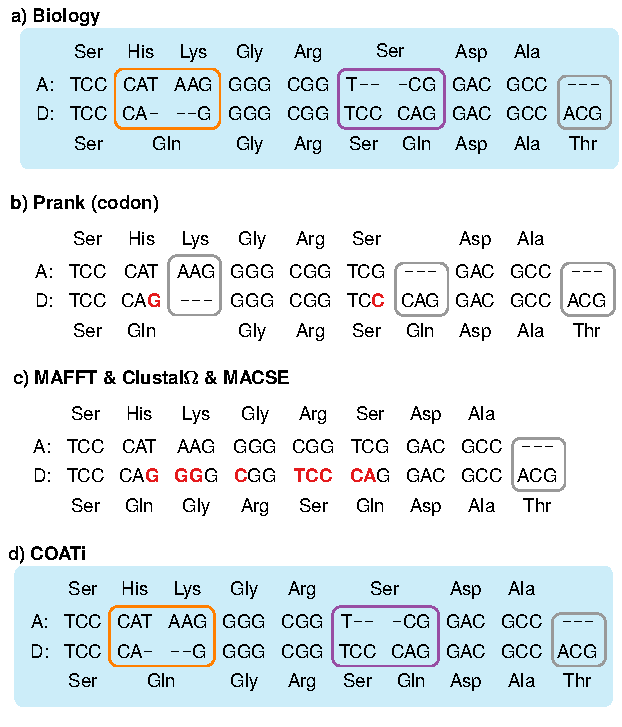
\includegraphics[scale=1]{figures/fig-aln.pdf}
    \par
    \caption{
        Standard algorithms produce suboptimal alignments.
        (a) shows the true alignment of an ancestor sequence (A) and a descendant sequence (D).
        (b--d) are the results of different aligners. Nucleotide mismatches are highlighted in red.---Notably, COATi is the only aligner able to retrieve the biological alignment in this example.---%
        %
        Indels in protein-coding sequences can be classified as having one of three difference phases and being one of two different types.
        Phases refer the the location of the gap with respect to the reading frame, while types refer to the consequence of the indel.
        Phase-1, phase-2, and phase-3 indels are shown in purple, orange, and gray respectively.
        Additionally, the orange indel is type-II (an amino-acid indel plus an amino-acid change) while the purple indel is type-I (an amino-acid indel only). The difference between in-frame and frameshift indels is not displayed.
        }
    \label{fig:aln}
\end{figure}

Bioinformatic pipelines need to be robust to variation in quality across genomic datasets because uncorrected errors in the alignment stage can lead to erroneous results in comparative and functional genomic studies \citep{estimates_schneider_2009, effect_fletcher_2010, hubisz2011error}.
While genomes for model organisms often get refined over many iterations and contain meticulously curated protein-coding sequences, 
genomes for non-model organisms might only receive partial curation and typically have lower quality sequences and annotations.
These genomes often lack the amount of sequencing data needed to fix artifacts, including missing exons, erroneous mutations, and indels \citep{jackman2018tigmint}.
%
When comparative and functional genomics studies include data from non-model organisms, care must be taken to identify and manage such artifacts; however,
current alignment methods are ill-equipped to handle common artifacts in genomic data, requiring costly curation practices that discard significant amounts of information.

To address current limitations of alignment software to accurately align protein-coding sequences, we present COATi, short for COdon-aware Alignment Transducer, a pairwise statistical aligner that incorporates evolutionary models for protein-coding sequences and is robust to artifacts present in modern genomic data sets.


\section*{Methods}

\subsection*{Statistical Alignment via Finite State Tranducers}

In statistical alignment, sequence alignments are scored based on a stochastic model, typically derived from molecular evolutionary processes \citep{Lunter2005-hk}. An advantage of statistical alignment is that its parameters are derived from biological processes, allowing them to be estimated directly from data or extracted from previous studies. While approaches vary, a statistical aligner for a pair of sequences, $X$ and $Y$, typically finds an alignment, $Aln$, that maximizes the joint probability $P(Aln, X, Y)$ or samples alignments from the posterior $P(Aln | X, Y)$. This is typically performed using pairwise hidden Markov models \citep[pair-HMMs;][]{bradley2007transducers}. Pair-HMMs are computational machines with two output tapes. Each tape represents one sequence, and a path through the pair-HMM represents an alignment of the two sequences. Conceptually, pair-HMMs generate two sequences from an unknown ancestor and can calculate the joint probability $P(Aln, X, Y)$ \citep{yoon_2009_hmm}.

While the use of pair-HMMs is ubiquitous in bioinformatics, they are limited to modeling the evolution of two related sequences from an unknown ancestor. As an alternative, finite-state transducers (FSTs, Fig.~\ref{fig:base-calling}) allow researchers to model the evolution of a descendant sequence from an ancestral sequence. FSTs are computational machines with one input tape and one output tape and provide similar benefits to pair-HMMs, while being more suitable for evolutionary models \citep{bradley2007transducers}. FSTs consume symbols from an input tape and emit symbols to an output tape based on the symbols consumed and the structure of the FST. Conceptually, FSTs generate a descendant sequence, $D$, from a known ancestor, $A$, and can calculate the conditional probability $P(Aln, D | A)$.

There are well-established algorithms for combining FSTs in different ways allowing the design of complex models by combining simpler FSTs, including concatenation, composition, intersection, union, and reversal \citep{bradley2007transducers,silvestre2021machine}. Specifically, composition is an algorithm to combine two FSTs by sending the output of one FST into the input of another, creating a new, more complex transducer \citep{mohri2005weighted}. Figure~\ref{fig:base-calling} illustrates how FSTs modeling sequencing errors (Fig.~\ref{fig:base-calling}a) and ambiguity (Fig.~\ref{fig:base-calling}b) can be combined via composition to produce an FST that does both (Fig.~\ref{fig:base-calling}c). Conceptually, composition creates an FST that generates a descendant sequence from a known ancestor via an unknown intermediate, $J$, and can calculate the conditional probability $P(D|A) = \sum_{J} P(D|J)P(J|A)$. 

\begin{figure}[!ht]
    \centering
    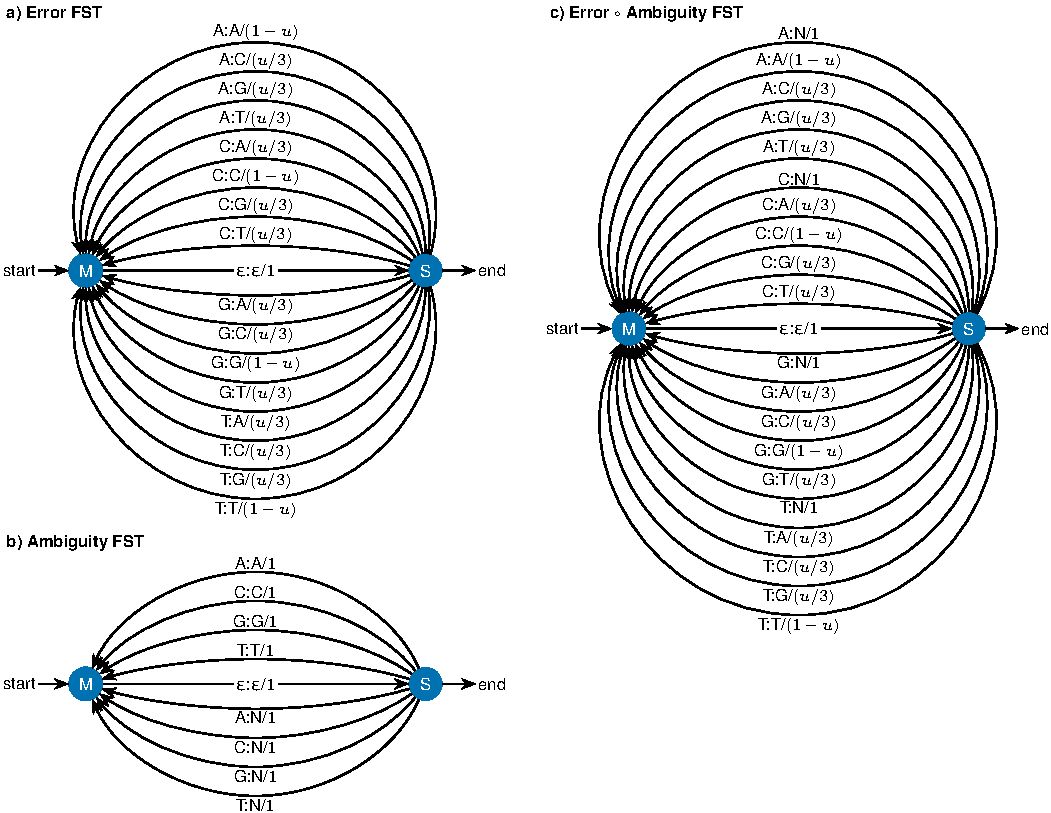
\includegraphics[width=\textwidth]{figures/fig-fst-base-calling-new.pdf}
    \caption[FSTs more the generation of sequences]{%
    Finite state transducers (FSTs) model the generation of an output sequences based on an input sequence.
    %
    (a) A graph of a probabilistic FST \citep{cotterell-etal-2014-stochastic} for base-calling errors using a Mealy-machine architecture, where parameter $u$ is the error rate. This graph contains two states (S and M) connected by arcs, with labels ``input symbols~:~output symbols~/~weight''. Arcs consume symbols from the input sequence and emit symbols to the output sequence. Weights describe the probability that an arc is taken given the input symbols. Epsilon (ε) is a special symbol denoting that no symbols were either consumed or emitted.
    %
    (b) An FST for matching sequences against ambiguous nucleotides (N). This FST is not a true probabilistic FST and cannot be used to simulate output sequences since it is missing a parameter to control how often Ns are added to the output sequence.
    %
    (c) An FST that results from the composition ($∘$ operation) of the Error FST with the Ambiguity FST. As with (b), this composed FST cannot be used to simulate output sequences; however, it does properly weight the ambiguous nucleotide N as representing any other symbol.
    %
    %Let $x$ be a symbol in the input of (a), $y$ be a symbol in the output of (b), and $z$ be a symbol in both the output of (a) and the input of (b). An arc in the composed FST (c) has an input symbol $x$, an output symbol $y$, and a weight that is the combination over $z$ of the aggregate weights of all $x$-$z$-$y$ arc pairs.
    %
    }\label{fig:base-calling}
\end{figure}

\subsection*{The COATi FST}

COATi aligns pairs of sequences using a statistical alignment model, which is implemented as a finite-state transducer derived from the composition of multiple FSTs, each representing a specific biological or technical process: (1) the codon substitution FST, (2) the indel FST, (3) the error FST, and (4) the ambiguity FST \citep[Figs.~\ref{fig:base-calling}--\ref{fig:coati-fst}; c.f.][]{holmes2001evolutionary}. We call this transducer the COATi FST. Codon substitution models are uncommon in sequence aligners, despite their extensive use in phylogenetics. COATi implements the Muse and Gaut (\citeyear{muse_gaut_1994}) codon model (codon-triplet-mg) and the Empirical Codon Model \citep[codon-triplet-ecm;][]{kosiol_ECM_2007}.
It also lets the user provide a codon substitution matrix. A key innovation of COATi is that it combines a codon substitution model with a nucleotide-based indel model, allowing gaps to occur both between and within codons \citep[c.f.][]{ranwez_macse_2011,ranwez_macse_2018}. This also allows the aligner to be robust against sequencing artifacts that produce sequences with disrupted reading frames.

Since codon substitution is the first process in COATi's model, the input sequence to the COATi FST must be compatible with a codon-substitution model, i.e.\ be a multiple of three nucleotides and not contain any ambiguous symbols or stop codons. The phases, reading frames, and amino-acid contexts of alignment columns is determined by the input sequence, and better alignments will be generated if the input is of high quality and free of artifacts. Depending on context, we may refer to the input sequence as the ``ancestral'' or ``reference'' sequence. In contrast, the output sequence must be compatible with the ambiguity FST, can be of any length, and can contain any nucleotides or ``N''. This allows COATi to align lower-quality sequences that may contain artifacts against a high-quality reference sequence. We may refer to the output sequence as the ``descendant'', ``non-reference'', or ``query'' sequence. The choice of which sequence is the input sequence and which sequence is the output sequence is left up to the user.

\begin{figure}[h!]
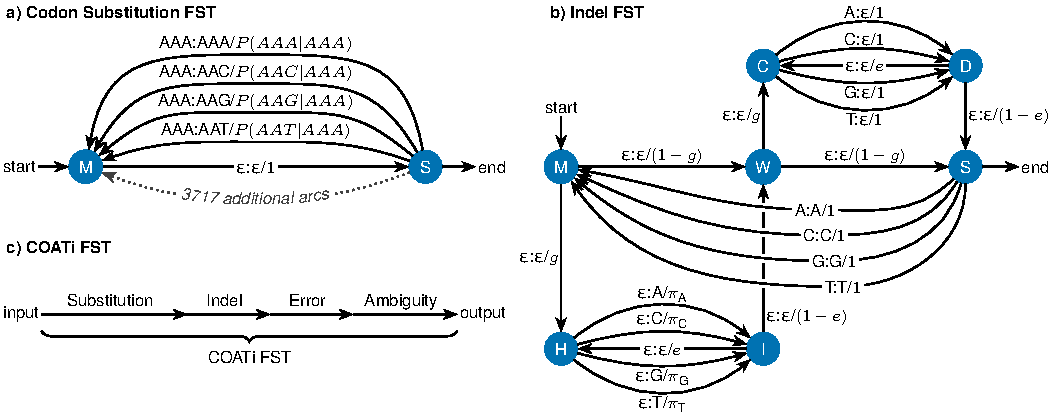
\includegraphics[width=\textwidth]{figures/fig-fst-coati.pdf}
\caption{The COATi FST is built from simpler FSTs via composition.
(a) The substitution FST encodes a $61 \times 61 $ codon substitution model with 3721 arcs from S to M. These arcs consume three nucleotides from the input tape and emit three nucleotides to the output tape. The weight of each arc is a conditional probability derived from a codon substitution model. See Fig.~\ref{fig:base-calling} for more details about reading this graph.
%
(b) The indel FST allows for insertions (H to I) and deletions (C to D). Here $g$ is the ``gap opening parameter'' and $e$ is the ``gap extension'' parameter.
Insertion arcs are weighted according to the codon model's stationary distribution of nucleotides, and deletion arcs have a weight of 1. This FST is structured such that if insertions and deletions are contiguous, insertions will precede deletions.
%
(c) The COATi FST is derived via composition from the codon substitution, indel, error, and ambiguity FSTs.
}
\label{fig:coati-fst}
\end{figure}

In order to use the COATi FST to align an output sequence against an input sequence, we first convert each sequence into an acceptor, represented as a linear transducer where the input and output symbols of each transition are identical and each transition represents one nucleotide of a sequence \citep{allauzen2007openfst}. By composing the input and output acceptors with the COATi FST, we generate a transducer of all possible alignments of the two sequences. Any path through this FST represents a pairwise alignment, while the shortest path (by weight) corresponds to the best alignment. If more that one optimal alignment exists, ties are broken according to the implementation of the shortest-path algorithm. All FST operations in COATi, including model development, composition, search for the shortest path, and other optimization algorithms, are performed using the C++ openFST library \citep{allauzen2007openfst}. An example of an FST-based alignment can be found in Supplementary Materials Figure 1.

\section*{The Marginal Model}

The COATi FST has a large state space to keep track of codon substitution rates when codons can be interspersed with indel events. This additional state space increases the computational complexity of the alignment algorithm. To reduce the runtime complexity of COATi, we have also developed an approximation of the COATi FST that can be implemented with standard dynamic programming techniques. This approximation uses a marginal substitution model where the output nucleotides are independent of one another and only depend on the input codon and position. This produces a $\left(61 \times 3 \right) \times 4$ substitution model and eliminates the need to track dependencies between output nucleotides.

A marginal substitution model is calculated from a standard substitution model by calculating the marginal probabilities that each ancestral codon produces specific descendant nucleotides at each reading frame position. Specifically, let
%
\[
P_\text{cod}\left( Y_1 = y_1, Y_2 = y_2, Y_3 = y_3 |
                   X_1 = x_1, X_2 = x_2, X_3 = x_3 \right)
\]
%
represent transition probabilities from a codon model, and
%
\[
P_\text{mar}\left(Y_p = y \middle| X_1 = x_1, X_2 = x_2, X_3 = x_3 \right)
=
\sum_{y_1, y_2, y_3} I(y_p = y)
P_\text{cod}\left( y_1, y_2, y_3 |
                   x_1, x_2, x_3 \right)
\]
%
represent the marginal transition probabilities, where $p \in \{1, 2, 3\}$ is the position of the descendant nucleotide relative to the ancestral reading frame and $I()$ is an indicator function. COATi contains marginal models for both Muse and Gaut (\citeyear{muse_gaut_1994}) or the Empirical Codon Model, resulting in the marginal models codon-marginal-mg and codon-marginal-ecm. These models emphasize the position in a codon where the substitution occurs, help restrict the effects of low-quality data in the descendant sequence, and allow more than one substitution per codon. In combination with the indel model, alignment using the marginal model is implemented using dynamic programming.

\subsection*{Empirical Dataset and Alignments}

Humans and gorillas are two closely related species with very different levels of genome curation. The human reference genome has been revised dozens of times and is currently on version GRCh38.p14, while the gorilla reference genome has only been revised a handful of times and is currently on version gorGor4 \citep[cf.\ ENSEMBL database v110;][]{ensembl_hubbard_2002}. Additionally significant levels of investment have been made to correctly identify and annotate human genes, while gorilla annotations have received limited support in comparison. Together, these reference genomes provide a good opportunity to compare COATi against other aligner as they offer one genome that is high-quality (human) and sister genome that is lower-quality (gorilla).

We used ENSEMBL database v110 \citep{ensembl_hubbard_2002} to create an empirical dataset of protein-coding sequences for both human genes and their gorilla orthologs. We first selected human protein-coding genes that belonged to the Consensus Coding Sequence Set, that were located on an autosomal chromosome, and that had a one-to-one gorilla ortholog. We selected the canonical isoform for both species and removed any pair in which the total nucleotide length was larger larger than 6,000 nucleotides. This resulted in 14,127 sequence pairs and corresponding FASTA files containing CDS sequences. Due to the way that canonical isoforms are identified, there is no guarantee that the isoforms are orthologous even though the genes are. Therefore, a subset of the sequence pairs in this dataset contain human and gorilla sequences with different exon compositions. We have made no attempt to correct these sequence pairs because in our experience genome-wide studies rarely control for such artifacts.

\paragraph{Alignment Methods.}

In order to compare COATi against other aligners, we evaluated five different alignment models: (1) COATi's FST model (i.e.\ codon-triplet-mg), (2) the amino-acid model of ClustalΩ via translation and reverse translation, (3) the amino-acid aware nucleotide model of MACSE, (4) the DNA model of MAFFT, and (5) the codon model of PRANK \citep{clustal_omega_sievers_2011,ranwez_macse_2018,katoh2013mafft,prank_loytynoja_2014}. 
COATi is not a symmetric pairwise aligner, as reference sequences are more constrained than non-reference sequences. In order to evaluate the importance of the choice for reference sequence, we also aligned sequences pairs using (6) COATi with gorilla sequences as the reference (i.e.\ COATI-rev). Together, these six methods allow us to evaluate both different alignment strategies and different software implementations. See Supplemental Materials for additional details, including results for COATi's marginal and ECM models.

We aligned our dataset of human-gorilla orthologs using all six alignment methods and calculated multiple biological and technical statistics on each alignment in order to compare how different alignment methods influence biological conclusions.
%
Additionally, we checked alignments to ensure that our pipeline did not introduce any artifacts into the results, including unexpected characters, empty columns, and aligned sequences of different lengths. We also generated checksums of our sequences to ensure that they were not modified during alignment.

\paragraph{Evolutionary Distances and Gaps.}

Alignment inference impacts the estimation of evolutionary distances. To quantify the impact of aligners on the estimation of evolutionary distances, we calculated Kimura's 2-parameter distance \citep[K2P;][]{kimura1980simple} for each sequence-pair and aligner combination. K2P corrects for multiple mutations at a site and takes into account differences in transition and transversion rates. It also assumes equal nucleotide frequencies and no variations in the rate of substitution across sites. While Kimura's 2-parameter distance is more suitable for non-coding sequences, it is straight forward to calculate and provides a quantitative measure of the evolutionary divergence between sequences. We used the R software package ape \citep{paradis2019ape} to calculate K2P distances.
%
Since aligners influence evolutionary distances based on their tendencies to insert gaps into sequences, we also quantified the lengths and phases of gaps introduced by each method as well as the fraction of nucleotides that are aligned against a gap.

\paragraph{Selection.}
Alignment inference also impacts the identification of genes that have experienced positive and negative selection. To evaluate the impact of aligners on selection identification, we estimated $K_S$ and $K_A$ statistics (also known as $d_s$ and $d_n$) for each estimated alignment. Briefly, $K_S$ is the number of substitutions per synonymous site and $K_A$ is the number of substitutions per non-synonymous site between two protein-coding sequences. We used the method developed by \cite{ka_ks_li_1993} and independently derived by \cite{Pamilo1993} to estimate these statistics as implemented in the R package seqinr \citep{seqinr}. 

Briefly, this method takes two aligned sequences and classifies the sites in each sequence as non-degenerate, two-fold degenerate, or four-fold degenerate based on the standard genetic code. A site is non-degenerate if 0/3 possible nucleotide changes to that site are synonymous, two-fold degenerate if 1/3 of the possible changes are synonymous, and four-fold degenerate if 3/3 possible changes are synonymous. (The rare three-fold degenerate sites are treated as two-fold degenerate in this method.) First the method calculates the average numbers of sites of each type in the sequence pair ($L_0$, $L_2$, and $L_4$). Next, following \cite{Li1985}, it uses Kimura's two-parameter model \citep{kimura1980simple} and the alignment to estimate the numbers of transitions ($A_i$) and transversions ($B_i$) that occurred per each $i$-th type. Using these statistics, \cite{ka_ks_li_1993} estimated $K_S$ and $K_A$ as
\begin{align*}
K_S &= \frac{L_2 A_2 + L_4 A_4}{L_2 + L_4} + B_4 &
K_A &= A_0 + \frac{L_0 B_0 + L_2 B_2}{L_0 + L_2}
\end{align*}

We considered any alignment to be showing evidence of positive selection if $K_A/K_S > 1$ and negative selection if $K_A/K_S < 1$. We estimated F\textsubscript{1} scores for both positive and negative selection by comparing estimated alignments to benchmark alignments. F\textsubscript{1} is the harmonic mean of precision and recall:
\[
F_1 = \frac{2 \text{TP}}{2 \text{TP} + \text{FP} + \text{FN}}
\]
where TP is the number of alignments that correctly predicted positive (or negative) selection, FP is the number of alignments that incorrectly predicted positive (or negative) selection, and FN is the number of alignments that incorrectly predicted the absence of positive (or negative) selection. F\textsubscript{1} allows us to measure how well aligners produce alignments that correctly identify the presence and absence of positive selection or negative selection.

\subsection*{Empirical Simulation Algorithm}

% 8263 gapless genes.
% 5864 gapped genes.

In order to compare COATi against other aligners on realistic datasets with known alignments, we developed a procedure to introduce realistic gap patterns into human-gorilla orthologous gene pairs that did not previous contain indels. Briefly, we downloaded 16000 human genes and their gorilla orthologs from the ENSEMBL database \citep{ensembl_hubbard_2002}. After downloading, we removed 2232 sequence-pairs longer than 6000 nucleotides and aligned the remaining pairs with the five alignment methods. Next we separated sequence pairs into two sets: (1) 6048 sequence pairs for which at least one aligner added gaps and (2) 7761 sequence pairs for which all five aligners did not introduce any gaps. We identified gap patterns from the sequence pairs that were aligned with gaps and randomly introduced them into the ungapped sequence pairs. We used an equal number of randomly sampled gap patterns from each aligner to produce a benchmark set of known alignments. The phases of gaps were preserved as were the spacings of any clusters of gaps. Segments of matches that were 99 nucleotides or longer were allowed to change length to accommodate the length of the ungapped sequence pair. (This criteria was recursively lowered if gap pattern did not fit the ungapped sequence pair.)

For example, consider the gapped alignment represented by the CIGAR string
%
``170M 3D 10M 6I 102M'' % Can use \allowbreak{} here instead of space
%
applied to an ungapped alignment of human and gorilla sequences that are 300 nucleotides long. First, we modify the CIGAR string to insert flexible lengths for any match segment that is 99 or more nucleotides long while preserving phase. This results in a new CIGAR string of
%
``101M *M 3D 10M 6I 99M *M'',
%
where * represents the locations that have flexible length. Considering only matches and deletions, this CIGAR string has 213 fixed nucleotides, leaving 87 nucleotides in the human sequence to be allocated to the flexible locations. Since there are two locations of flexible length, we draw one random break point uniformly while maintaining phase, producing the final CIGAR string of
%
``101M 9M 3D 10M 6I 99M 78M'',
%
which is used to add gaps into the target, ungapped sequence pair.
To apply deletions, we remove the corresponding nucleotides from the gorilla sequence, and to apply insertions, we add random nucleotides according to their stationary frequency to the gorilla sequence at the corresponding locations. The human sequence is left unchanged.


% The simulation algorithm can introduce a pairwise alignment pattern to any two nucleotide sequences of equal length. The alignment pattern is given as a CIGAR string (Compact Idiosyncratic Gapped Alignment Report), a format commonly used to summarize aligned reads to a reference genome. Assigning one of the sequences as the reference, to distinguish between insertions and deletions, CIGAR strings can also summarize pairwise alignments by grouping the number of contiguous matches or mismatches `M', deletions `D', and insertions `I'. The resulting pattern combines these letters preceded by the number of characters for each section as they appear in the alignment. This pattern is introduced by replacing nucleotides with gaps as indicated by deletions on one sequence and randomly introducing residues where the CIGAR strings indicated insertions.

% Several safety checks are in place to ensure the algorithm runs correctly and the result is accurate. The assertions are divided into checking lengths and maintaining the reading frame of each section. The simulation can fail if the length of the sequences is different or if, without counting insertions, the length of the pattern to be inserted is longer. In addition, maintaining the phases of each section in the CIGAR string is important to avoid introducing errors such as frameshifts. 

% I created the benchmark of alignments by using an equal number of randomly sampled gap patterns from each aligner.
% % After creating the dataset, I removed the gaps and measured how well different aligners were able to retrieve the true alignments.
% I used the dataset to evaluate the accuracy of COATi and a suite of popular aligners spanning various alignment methods:
% Clustal$\Omega$ v1.2.4 \citep{clustal_omega_sievers_2011},
% MACSE v2.06 \citep{ranwez_macse_2011}, MAFFT v7.505
% \citep{katoh2013mafft}, and PRANK v.150803 \citep{prank_loytynoja_2014}.

\subsection*{Alignment Accuracy Measures}

We used multiple statistics to to quantify the similarity between each alignment in the benchmark and the corresponding output obtained by the different tools.

Alignment error also negatively impacts the estimation of evolutionary distances and phylogenetic trees. To quantify the impact of aligners on the estimation of evolutionary distances, we compared Kimura's 2-parameter distance \citep[K2P;][]{kimura1980simple} calculated for the estimated and benchmark alignments. 

Alignment error negatively impacts the identification of genes that have experienced positive and negative selection.

Alignment error negatively impacts the identification of genes that have experienced positive and negative selection. To evaluate the impact of aligners on selection identification, we estimated $K_S$ and $K_A$ statistics (also known as $d_s$ and $d_n$) for each estimated alignment and compared them to the benchmark alignment. 

\paragraph{Alignment Error.}
To quantify the error between estimated alignments and the benchmark alignments, we used the alignment error metric $d_{seq}$ \citep{metrics_blackburne_whelan_2011}. Intuitively, $d_{seq}$ ranges between zero and one and can be interpreted as the fraction of nucleotides in the sequence pair that are aligned differently between estimated and benchmark alignments. This metric summarizes each alignment by building homology sets for each nucleotide in the sequence pair. Briefly, if an alignment column contains position $i$ from the first sequence and position $j$ from the second sequence, then $\{j\}$ is the homology set for position $i$ in the first sequence and $\{i\}$ is the homology set for position $j$ in the second sequence. If a position is aligned against a gap, then its homology set is simply $\{\text{gap}\}$. This treats all gaps equally as the location of the gap is not recorded. Finally, $d_{seq}$ is calculated  between an estimated and a benchmark alignment as the average, normalized Hamming distance between the homology sets for each nucleotide in the sequence pair. See \cite{metrics_blackburne_whelan_2011} for further details.

% The computation of $d_{seq}$ involves characterizing the gaps present in the alignment. Then, a site-wise homology set $H(A)^i_j$ is calculated for each alignment $A$, sequence $i$, and character $j$. The distance between two alignments $A$ and $B$ is the average across all characters of the symmetric difference (or Hamming distance), represented as `$\triangle$' between homology sets over the length of such sets:

% \begin{equation}
% d(A,B) = \frac{1}{c} \sum_i \sum_j \frac{|H(A)^i_j \triangle H(B)^i_j|}{|H(A)^i_j|+|H(B)^i_j|}
% \end{equation}

% \noindent where $c$ is the sum of the sequence lengths.

\paragraph{Perfect, Imperfect, and Best Alignments.}
We quantified the number of perfect, imperfect and best alignments each aligner produced. We define perfect alignments as alignments with a distance of zero to their benchmark alignment ($d_{seq} = 0$) or any alignment that is evolutionary equivalent to an alignment with a distance of zero. Equivalency was included in our definition of perfect alignments to prevent the manner by which aligners break ties between multiple optimal alignments from impacting our results. Evolutionary equivalence was determined by scoring alignments using COATi's marginal model. Any alignment that had a score which matched the score of its benchmark alignment was considered perfect even if its distance to the benchmark was greater than zero.
%
Imperfect alignments are defined as alignments that are not perfect when another method successfully produces a perfect alignment for the same pair of sequences.
%
Best alignments are the alignments that the lowest distance $d_{seq}$ to the true alignment, including ties.
%
Taken together, these three statistics not only allow a direct comparison of aligners but also expose instances where all aligners fall short of achieving a perfect result.

% \cyan{The first sentence intro is a good idea, but rewrite!}
% Sequencing artifacts and errors made in alignment can lead to inaccurate results in genomics. This is especially true in studies of positive selection and positively selected genes.

% Ks and Ka are, respectively, the number of substitutions per synonymous site and per non-synonymous site between two protein-coding genes.



% First, this method takes two aligned homologous protein-coding sequences and classifies the nucleotide sites in a sequence as nondegenerate, twofold degenerate, and fourfold degenerate. A site is nondegenerate if all possible changes at that site are nonsynonymous, twofold degenerate if one of the three possible changes is synonymous, and fourfold degenerate if all possible changes are synonymous. Second, the nucleotide changes between the two sequences are counted and divided as transitional (A$\leftrightarrow$G, C$\leftrightarrow$T) and transversional (\{A, G\}$\leftrightarrow$\{C, T\}). Third, the Kimura two-parameter distance \citep{kimura1980simple} is used to estimate the number of transitions and transversions per site type (nondegenerate, twofold degenerate, and fourfold degenerate), which is used as a correction factor for multiple hits. Finally, $k_s$ is the estimate of the average transitional rate at twofold and fourfold degenerate sites, and $k_a$ is the estimate of the average transversional rate at nondegenerate and twofold sites. In the results, these metrics are reported as the F$_1$ score, which is the harmonic mean of precision (true positives over total positives) and recall (true positives over true positives and false negatives). This score ranges between 0 and 1, with a score of 1 representing a perfect result.


% e compared the estimated evolutionary distance between the reference and inferred alignments using the Kimura's 2-parameter distance \citep{kimura1980simple}. The calculation of the Kimura 2-parameter model involves considering the rates of nucleotide transitions and transversions. The formula used for distance calculation is $D = -0.5 \cdot \log((1 - 2P - Q) \cdot \sqrt{1 - 2Q})$, where $P$ represents the proportion of transitional substitutions and $Q$ represents the proportion of transversional substitutions. 

\section*{Results}

\paragraph{Empirical Data and Alignments.}

We generated 14,127 sequence pairs containing the coding sequences of a human gene and the orthologous gorilla gene. 22 human sequences contained early stop codons. These were not artifacts, but rather UGA codons which encoded for selenocysteine. 1 human sequence had a length that was not a multiple of 3, and no human sequences contained ambiguous nucleotides. Conversely, no gorilla sequences contained early stop codons (i.e.\ proteins containing selenocysteines were improperly annotated). 20 gorilla sequences had lengths that were not multiples of 3, and 173 sequences contained ambiguous nucleotides.

COATi was not able to align 23 sequence pairs, PRANK was not able to align 24 sequence pairs, and COATi-rev was not able to align 193 sequence pairs. MAFFT, MACSE, and ClustalΩ were able to align all sequence pairs, although the latter received some help from our wrapper script.

\begin{figure}[h!]
    \centering%
    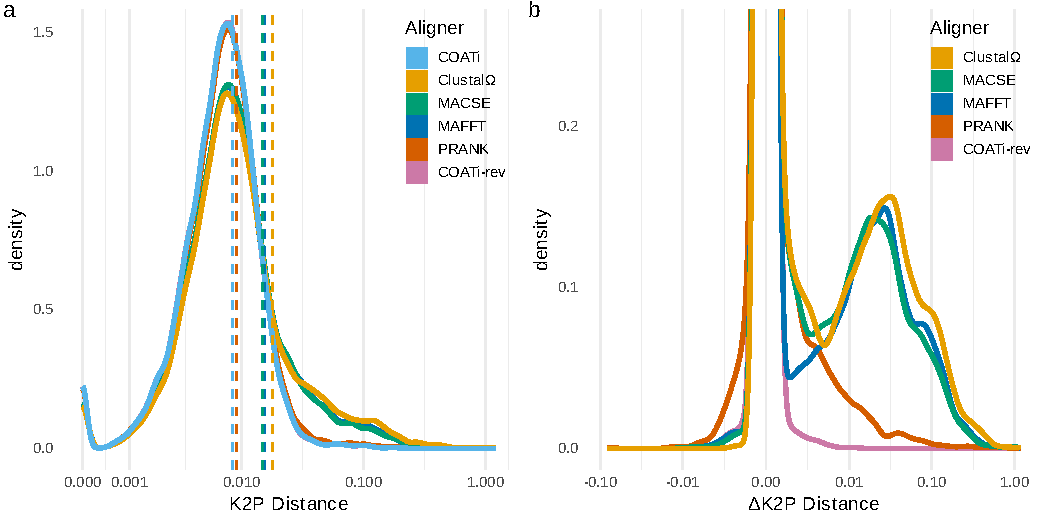
\includegraphics{figures/fig-k2p-empirical.pdf}
    \par
    \caption{COATi's alignments produce biologically reasonable evolutionary distances. (a) The distribution of K2P distances inferred from alignments generated by each method. The averages of each distribution are indicated by vertical lines. The averages are COATi = 0.0084, ClustalΩ = 0.0178, MACSE = 0.0149, MAFFT = 0.0154, PRANK = 0.0092, and COATi-rev = 0.0084. (b) The distribution of the differences between distances inferred by COATi and other methods. The X-axes of both plots have been pseudo-log transformed using the inverse hyperbolic sine.}
    \label{fig:k2p-empirical}
\end{figure}

% Wilcoxon signed rank test
% coati vs rev-coati: p-value: 0.4212 (two.sided)
% coati vs prank: p-value: < 2.2e-16 (less)
% coati vs macse: p-value: < 2.2e-16 (less)
% coati vs mafft: p-value: < 2.2e-16 (less)
% coati vs clustalo: p-value: < 2.2e-16 (less)

\section*{Discussion}
% Using 16000 human genes and their gorilla orthologs from the ENSEMBL
% database \citembe{ensembl_hubbard_2002}, we simulated a data set of pairwise
% alignments with empirical gap patterns.
% We used the data set to evaluate the accuracy of COATi and a suite of popular aligners spanning multiple alignment methods:
% Clustal$\Omega$ v1.2.4 \citembe{clustal_omega_sievers_2011},
% MACSE v2.06 \citembe{ranwez_macse_2011}, MAFFT v7.505
% \citembe{katoh2013mafft}, and PRANK v.150803 \citembe{prank_loytynoja_2014}.

% After downloading, we removed 2232 sequence-pairs longer than 6000 nucleotides and then aligned the remaining pairs with all five methods.
% At least one aligner added gaps to 6048 sequence pairs, and no aligner added gaps to 7719 sequence pairs.
% We then randomly introduced gap patterns extracted from all five methods into the ungapped sequence pairs to generate the benchmark alignments.
% The accuracy of inferred alignments compared to the benchmarks was measured using \citeauthor{metrics_blackburne_whelan_2011}'s \citeyearpar{metrics_blackburne_whelan_2011} distance metric, $d_{seq}$.
% Additionally, because different alignments may be evolutionary equivalent, we scored alignments using the codon-marginal-mg model, and any alignment that had the same score as the benchmark alignment was considered equivalent to the benchmark alignment.
% The accuracy of identifying positive and negative selection was calculated using the $F_1$ score by estimating $k_s$ and $k_a$ statistics
% \citembe{ka_ks_li_1993} (Supplementary Methods).
% The $F_1$ score evaluates the accuracy of a model by assigning equal importance to precision and recall, and ranges between 0 and 1, with a score of 1 representing a perfect result.

COATi obtained better results compared to a wide variety of alignment strategies. It was significantly more accurate (lower $d_{seq}$) at inferring the empirically simulated alignments compared to other methods; all p-values were less than $1.3 \cdot 10^{-76}$ according to the one-tailed, paired Wilcoxon signed-rank tests (Supplementary Materials Figure 1). Notably, the average alignment error of the second best protocol was six times larger than COATi's. In addition, COATi produced more perfect alignments, less imperfect alignments, and more accurately inferred events of positive and negative selection (Table \ref{table:comp}). Furthermore, the estimated evolutionary divergence from the alignments retrieved by COATi was substantially less overestimated than other methods (Table \ref{table:comp}, Supplemental Materials Figure 8).

Aligning sequences using amino-acid translation via ClustalΩ obtained the highest average alignment error and also had difficulties correctly identifying positive selection and estimating evolutionary distances. These results are not surprising because alignments in amino-acid space only permit phase-3 gaps and are sensitive to frameshift artifacts, which inflate divergence estimates and impact selection detection. Conversely, we obtained better results when aligning in nucleotide space using both amino-acid aware MACSE and amino-acid agnostic MAFFT. These results indicate that aligning protein-coding sequences in nucleotide space works reasonably well if the sequences come from closely related species, such as humans and gorillas, as it supports all three gap phases and is robust to frameshift artifacts. If the sequences were further apart, we predict that amino-acid agnostic approaches would begin to produce unreasonable alignments. And finally, our PRANK protocol used a codon substitution model which should have been an improvement over both amino-acid and nucleotide models; however, PRANK's codon model only permits phase-3 gaps and is very sensitive to frameshift artifacts. In fact, PRANK refuses to align any sequence using a codon model if its length is not a multiple of three.

% Software comparison table
\begin{table}[!ht]
\centering
% \begin{table}[h!]
% \begin{adjustbox}{width=\columnwidth,center}
\definecolor{bestcolor}{RGB}{230,230,230}

\begingroup\centering
\begin{tabular}{r|ccccc}
      & \textbf{COATi} & \textbf{MAFFT} & \textbf{PRANK\footnotesize{*}} & \textbf{MACSE} & \textbf{Clustal$\Omega$}\\
\hline
Method    & Trip-MG & DNA & Codon & DNA+AA & AA\\[2pt]
%\hline
Avg alignment error ($d_{seq}$) & \cellcolor{bestcolor}0.00214 & 0.01392 & 0.02001 & 0.01351 & 0.02691\\
Perfect alignments & \cellcolor{bestcolor}5722 & 5408 & 4706 & 2860 & 2937\\
Best alignments & \cellcolor{bestcolor}5152 & 4833 & 4748 & 3754 & 2595\\
Imperfect alignments & \cellcolor{bestcolor}1066 & 1380 & 2082 & 3928 & 3851\\
% \hline
F1 score of positive selection & \cellcolor{bestcolor}98.2\pct & 86.1\pct & 88.4\pct & 81.2\pct & 71.0\pct \\
F1 score of negative selection & \cellcolor{bestcolor}99.8\pct & 98.6\pct & 98.8\pct & 98.3\pct & 97.0\pct
\end{tabular}
\par\endgroup
% \end{adjustbox}
% \end{table}


 \vspace{1mm}
 \footnotesize{\textsuperscript{*}PRANK produced 42 empty alignments, calculations are based on 7719 alignments.}
 \caption{COATi generates better alignments than other alignment algorithms. Results of COATi, PRANK, MAFFT, Clustal$\Omega$, and MACSE aligning 7761 empirically simulated sequence pairs. Best alignments have the lowest $d_{seq}$ (including ties), perfect alignments have the same score as the true alignment, and imperfect alignments have a different score than the true alignment when at least one method found a perfect alignment.}
 \label{table:comp}
\end{table}

COATi is not a symmetric pairwise aligner, as reference sequences are more constrained than non-reference sequences. To test how well COATi performs when the roles of sequences are reversed, we realigned the 7761 benchmark sequence alignments using gorilla as the reference. Notably, COATi was only able to align 4003 sequence pairs due to the presence of early stop codons or other artifacts in 3758 simulated gorilla sequences. While the simulation algorithm prevents disrupting the reading frame and introducing frameshifts, it does not prevent early stop codons from being formed in the descendant sequence. Despite this limitation, we analyzed the 4003 alignments and compared the results across methods, including COATi using the human sequence as the reference. The results show a decrease, albeit small, in accuracy across all metrics when the low-quality sequence is used as the reference in comparison to the reverse (Supplementary Materials Tab. 6). However, the results for COATi continue to be a significant improvement over other aligners.

COATi uses finite-state transducers to align pairs of sequences using a codon-aware statistical model. While COATi has multiple modes and models, here we have focused on evaluating the utility of COATi FST for estimating pairwise alignments. We have shown that COATi offers a biologically significant improvement over other methods when aligning pairs of sequences separated by short evolutionary distances in the presence of genomic artifacts. In other work, we have begun to explore application of COATi to more divergent sequences and the accuracy of the marginal approximation of the COATi FST \citep{garcia2023dissertation}. 

COATi is under active development. We plan on extending it to support more complex gap models, e.g.\ mixtures of single-nucleotide and triple-nucleotide indel models and weighing gap openings to reflect known selection on indel phases \citep{zhu2022profiling}. We plan on improving its multiple-sequence alignment and alignment sampling capabilities, as well as implement new models for aligning long-read sequences of genes against reference genomes. Our goal is to develop COATi into a user-friendly suite of tools that will allow researchers to analyze more data with higher accuracy and facilitate the study of important biological processes that shape genomic data.

\section*{Availability}
The source code for COATi, along with documentation, is freely available on GitHub: \url{https://github.com/CartwrightLab/coati} and is implemented in C++. Additional information, code, and workflows to replicate the analysis can be found on GitHub: \url{https://github.com/jgarciamesa/coati-testing}.

% \section*{Supplementary information}

\section*{Acknowledgments}

This research was funded by NSF award DBI-1929850.
%
The authors would like to thank Profs.\ Marco Mangone, Ted Pavlic, Banu Oskan, Jay Taylor, and Jeremy Wideman for their helpful support on two separate PhD dissertation projects. The authors would also like to thank the associate editor and two reviewers for their helpful comments on earlier versions of this manuscript.

\noindent \textit{Conflict of interest:} none declared.

% \section{References}
\bibliographystyle{mbe}%
\setlength{\bibhang}{0pt}
\bibliography{alignpair_letter.bib}

\nolinenumbers

\end{document}
